\documentclass{article}
\usepackage[margin=1.5cm,bottom=2cm]{geometry}
\usepackage{fancyhdr}
\usepackage{graphicx}
\usepackage{amsmath}
\usepackage{enumitem}
\pagestyle{fancy}

\begin{document}
\fancyhead[L]{ 
\includegraphics[width=2cm]{au_logo.png} }
\fancyhead[R]{PHYS 4220: Computational Physics}
\fancyfoot[C]{\thepage}
\vspace*{0cm}
\begin{center}
	{\LARGE \textbf{Homework 3}}\\
	\vspace{0.25cm}
	{\Large Due: Wednesday, November 4}
\end{center}

\newcommand{\textbook}{\textit{Giordano}}

{\textbf{Lagrangian Mechanics Tutorial}}
\begin{enumerate}
	\item Consider the system consisting of a mass $m$ suspended at the end of a spring with equilibrium length $\ell$. This problem will guide you through the process of deriving the equations of motion for the mass.
	\begin{figure}[ht!]
		\centering
		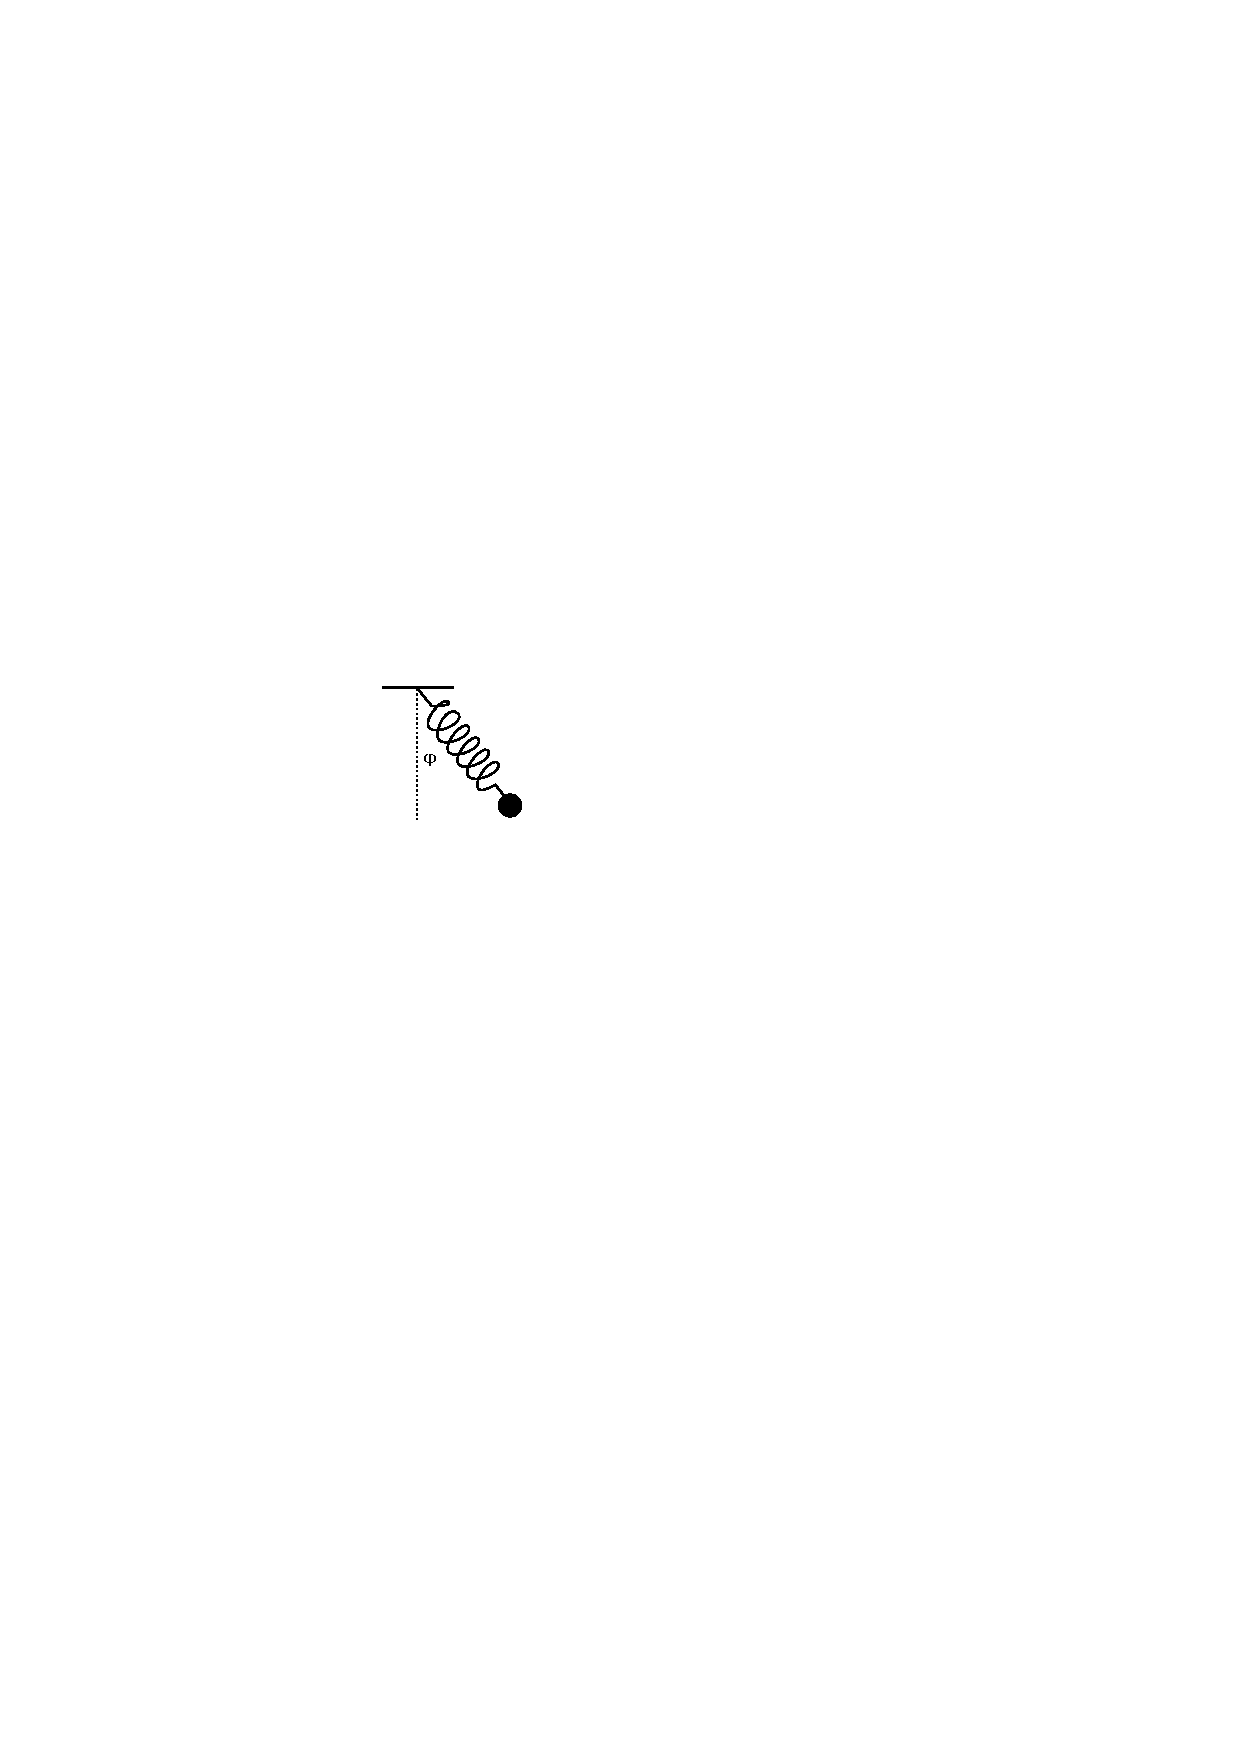
\includegraphics[width=0.2\textwidth]{spring}
	\end{figure}
	\begin{enumerate}
		\item Write the Lagrangian $\mathcal{L}=T-U$:
		\begin{enumerate}
			\item[--] In terms of $r$ and $\phi$, write the vector $\vec{r}$ which describes the position of the mass.\\ \textit{Hint: Choose the two coordinates $r$ and $\phi$ to parameterize the position of the mass. Let the origin be the point at which the spring attaches to the ceiling: so $r$ is the absolute distance from the origin to the mass, $\phi$ is the angle from the vertical as shown in the diagram.}
			\item[--] By taking the time derivative of $\vec{r}$ from above, write the kinetic energy $T=\frac{1}{2}mv^2=\frac{1}{2}m\left(\dot{\vec{r}}\cdot\dot{\vec{r}}\right)$
			\item[--] Write the total potential energy of the system, which is simply the potential energy due to gravity plus the potential energy stored in the spring.
			\item[--] Write the Lagrangian $\mathcal{L}=T-U$
		\end{enumerate}
		\item Use the Euler-Lagrange equations to obtain the equation of motion for both the $r$ and $\phi$ coordinate:
		\begin{enumerate}
			\item[--] For the $r$ coordinate: 
			\begin{equation*}
				\frac{\partial \mathcal{L}}{\partial r} = \frac{d}{dt}\left(\frac{\partial\mathcal{L}}{\partial \dot{r}}\right)
			\end{equation*} 
			\item[--] For the $\phi$ coordinate:
			\begin{equation*}
				\frac{\partial \mathcal{L}}{\partial \phi} = \frac{d}{dt}\left(\frac{\partial\mathcal{L}}{\partial \dot{\phi}}\right)
			\end{equation*} 
		\end{enumerate}
	\item Show that in the limit of an extremely rigid spring (i.e. $\ddot{r}=\dot{r}=0$) your equations simplify to the equation of motion for a simple pendulum.
	\item Show that if there is no motion in the $\phi$ direction ($\ddot{\phi}=\dot{\phi}=0$), then the result is simple harmonic motion in the vertical direction.
	\end{enumerate}
\end{enumerate}

{\textbf{Spring Force Gravity}}
\begin{enumerate}[resume]
	\item Consider an alternative Universe, where instead of $\vec{F}=-\frac{Gm_1m_2}{r^2}\hat{r}$, the gravitational force is: 
	\begin{equation*}
		\vec{F}=-G'm_1m_2r\hat{r}
	\end{equation*}
	In this scenario, the potential energy $U$ of the gravitational interaction is:
	\begin{equation*}
		U=G'm_1m_2r^2
	\end{equation*}
	For the following questions, apply the same methods we used in class for a central force, substituting the above form of the potential energy.
	\begin{enumerate}
		\item What is the equation of motion for the radial coordinate $r$?
		\item What is the equilibrium orbit $r_0$?
		\item Normalize your equation from (a) and write a program to numerically solve it. Plot the motion (x vs y) for several different initial conditions. Do the bounded orbits close on themselves to form circles and ellipses, as they do with Newtonian gravity?
		\item Are unbounded orbits possible in this alternative Universe?
	\end{enumerate}
\end{enumerate}
\end{document}